\documentclass{article}
\usepackage{tikz}
\usetikzlibrary{arrows.meta,positioning,calc,shapes.geometric}
\pagestyle{empty}
\begin{document}
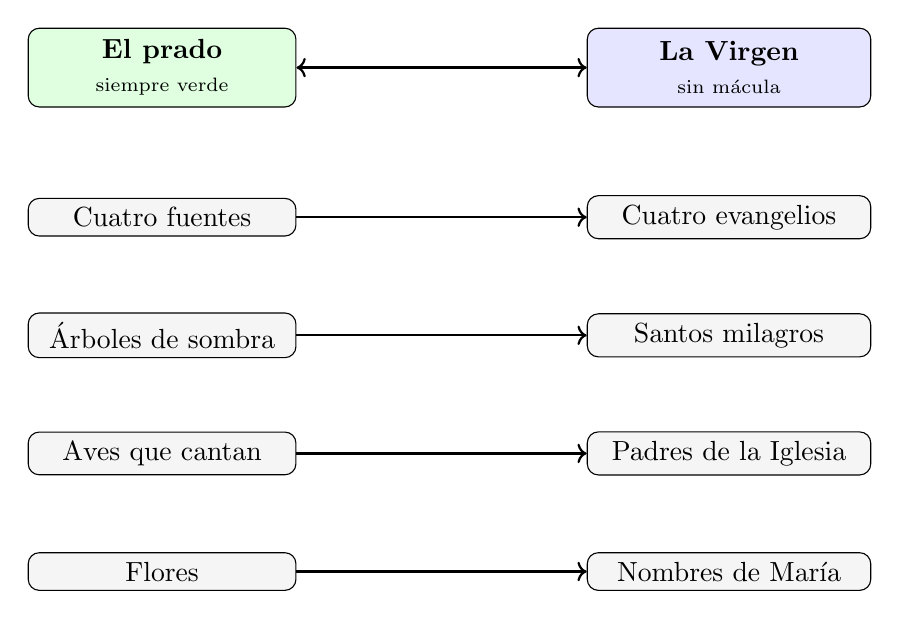
\begin{tikzpicture}
\tikzset{every node/.append style={align=center}}

\node[draw, rounded corners, fill=green!12, minimum width=3.4cm, minimum height=1.0cm, align=center] (p) at (0,0) {\textbf{El prado}\\ \scriptsize siempre verde};
\node[draw, rounded corners, fill=blue!10, minimum width=3.6cm, minimum height=1.0cm, align=center] (v) at (7.2,0) {\textbf{La Virgen}\\ \scriptsize sin mácula};
\draw[<->, thick] (p) -- (v);
\node[draw, rounded corners, fill=gray!8, minimum width=3.4cm, align=center] (f) at (0,-1.9) {Cuatro fuentes};
\node[draw, rounded corners, fill=gray!8, minimum width=3.6cm, align=center] (e) at (7.2,-1.9) {Cuatro evangelios};
\node[draw, rounded corners, fill=gray!8, minimum width=3.4cm, align=center] (a) at (0,-3.4) {Árboles de sombra};
\node[draw, rounded corners, fill=gray!8, minimum width=3.6cm, align=center] (m) at (7.2,-3.4) {Santos milagros};
\node[draw, rounded corners, fill=gray!8, minimum width=3.4cm, align=center] (b) at (0,-4.9) {Aves que cantan};
\node[draw, rounded corners, fill=gray!8, minimum width=3.6cm, align=center] (d) at (7.2,-4.9) {Padres de la Iglesia};
\node[draw, rounded corners, fill=gray!8, minimum width=3.4cm, align=center] (l) at (0,-6.4) {Flores};
\node[draw, rounded corners, fill=gray!8, minimum width=3.6cm, align=center] (n) at (7.2,-6.4) {Nombres de María};
\foreach \x/\y in {f/e,a/m,b/d,l/n} \draw[->, thick] (\x) -- (\y);

\end{tikzpicture}
\end{document}
